\section{Processi Organizzativi}

\subsection{Gestione della comunicazione}
In questa sezione vengono esposte le norme che dovranno essere seguite per comunicare tra le varie parti (proponente,  committenti,  membri  del  gruppo DPCM 2077).
\subsubsection{Comunicazioni interne}

Questa sezione riguarda le norme da rispettare per la comunicazione all'interno del gruppo DPCM 2077. Per le comunicazioni interne al gruppo è stato inizialmente adottata la nota applicazione \glock{Telegram}.
È stato creato un gruppo contenente i 7 membri di DPCM 2077.
In seguito si è deciso di affiancare a Telegram anche l'applicazione \glock{Discord}.
Discord consente di inviare messaggi, fare chiamate vocali e di condividere lo schermo.
All'interno dell'applicazione sono stati creati vari sotto-canali riguardanti i vari documenti da redigere (e.g. glossario-aggiornamento, piano-di-progetto e norme-di-progetto)
per poter scambiare messaggi solo con le persone coinvolte nella redazione di un certo documento.
Per video-chiamate, oltre a \glock{Zoom} è stato usato l'applicativo \glock{Meet} di Google per una maggiore semplicità di utilizzo.

Canali tematici predisposti all'interno di Discord:
\begin{itemize}
\item{regole-generali: per discutere di ciò che riguarda l’organizzazione generale del progetto, la scelta degli strumenti di lavoro, le decisioni da prendere in modo rapido, senza bisogno di indire una riunione o un incontro  su Zoom / Meet;}
\item{help-github: per poter chiedere aiuto nel caso di problemi durante il versionamento dei file;}
\item{off-topic: dove discutere liberamente di tutto ciò che non concerne strettamente il progetto e/o lo sviluppo del prodotto;}
\item{glossario-aggiornamento: per segnalare nuove parole da aggiungere al Glossario;}
\item{piano-di-progetto: per poter discutere riguardo al documento esterno Piano di Progetto;}
\item{norme-di-progetto: per poter discutere riguardo al documento interno Norme di Progetto;}
\item{analisi-dei-requisiti: per poter discutere riguardo al documento esterno Analisi dei requisiti.}
\end{itemize}
I membri del gruppo DPCM 2077 sono tenuti a comunicare tra loro, rispettando le tematiche dei canali preposti. Nel caso volessero portare all’attenzione di un particolare membro del gruppo un certo messaggio sono tenuti ad usare
il comando @userName.
Invece usando il comando @everyone è possibile portare il messaggio all'attenzione di tutti.
Le riunioni possono essere svolte solo tramite canali telematici, a causa del propagarsi della pandemia, e quindi non in presenza fisica.

\subsubsection{Comunicazioni esterne}
Questa sottosezione riguarda le norme alle quali attenersi per comunicare con soggetti esterni a DPCM 2077.
Soggetti esterni individuati:
\begin{itemize}
\item{la proponente \glock{Imola Informatica}. È possibile comunicare con il Dr. Lorenzo Patera e il Dr. Luca Cappelletti che hanno contribuito a creare il capitolato d'appalto;}
\item{i committenti Prof.~Tullio Prof.~Vardanega, ai quali verrà fornita tutta la documentazione necessaria a sostenere con successo le varie revisioni di progetto, e con i quali si intende creare un rapporto che migliori 
di continuo i processi e le strategie adottate.}
\end{itemize}

\paragraph{Comunicazioni esterne scritte}
Le comunicazioni esterne scritte devono avvenire attraverso l’utilizzo dell’indirizzo email del gruppo: \textbf{dpcm2077@gmail.com}. 
Nel caso di un messaggio da inviare rivolto a più destinatari, nel campo “A:” va indicato il destinatario principale, e nel campo “CC:” vanno indicati tutti gli altri destinatari (mettere in copia).
Le email dovranno essere scritte dal Responsabile di Progetto che dovrà avere cura di includere il logo del gruppo e di apporre la propria firma.

\subsection{Riunioni}
Questa sezione ha lo scopo di definire le stesse e le loro modalità di svolgimento. Nelle riunioni è il responsabile che convoca la riunione con scadenza settimanale, stende l'o.d.g, assegnando la giusta priorità ai vari punti da discutere e conduce / modera la discussione. Se qualcuno del gruppo vuole proporre un argomento contatta i responsabili prima della riunione, che lo inseriranno nell'o.d.g e gli daranno la priorità corretta e lo spazio se c'è. Un componente nominato segretario redige solo il verbale.
In Google drive è stato creato un o.d.g. temporaneo dove i componenti di DPCM 2077 possono vedere l’o.d.g. della riunione in anticipo. Inoltre è stato creato un documento dove raccogliere le decisioni prese nel corso della settimana, tra una riunione e la successiva, per non perderne traccia. Esse saranno validate alla prima riunione utile. È compito del responsabile tenere aggiornati l'o.d.g. temporaneo e il tracciamento delle decisioni settimanali.
\subsubsection{Verbali di riunione}
Nello svolgimento delle riunioni è compito del segretario nominato (a rotazione) redigere il verbale di riunione secondo le seguenti indicazioni:
\begin{itemize}
\item{\textbf{introduzione}, questa sezione contiene:}
	\begin{itemize}
	\item{luogo: ad esempio, videoconferenza su Meet;}
	\item{data: nel formato AAAA-MM-GG, ad esempio 2020-12-14;}
	\item{ora di inizio:  nel formato ventiquattro ore, ad es. 15:30;}
	\item{ora di fine:  nel formato ventiquattro ore, ad es. 15:30;}
	\item{ordine del giorno: punti discussi sotto forma di elenco puntato.}
	\end{itemize}
\item{\textbf{Presenze}}
	\begin{itemize}
	\item{presenti: nominativi dei componenti presenti;}
	\item{assenti: nominativi dei componenti eventualmente assenti;}
	\end{itemize}
\item{\textbf{svolgimento}: contiene le annotazioni circa gli argomenti discussi e non discussi tra quelli presenti nell’Ordine del giorno, le decisioni prese o non prese e le motivazioni che hanno portato a tali decisioni.}
\item{\textbf{tracciamento delle decisioni}: riepilogo in in forma tabellare delle decisioni prese nel corso della riunione;}
\end{itemize}
\textbf{Nomenclatura dei verbali: } i verbali interni dovranno avere come nome: \textbf{VI\_AAAA-MM-GG\_v1.0.0}, ad esempio VI\_2021-01-11\_v1.0.0 e quelli esterni: \textbf{VE\_AAAA-MM-GG\_v1.0.0}. v1.0.0 è un esempio di versione.\\
\textbf{Modalità di conservazione dei verbali:} i verbali sono redatti in \LaTeX, i verbali interni sono conservati nella cartella \textbf{interni} nel repository \glock{GitHub} contentente la documentazione, e quelli esterni nella cartella \textbf{esterni}.

\subsubsection{Riunioni interne}
Alle riunioni interne partecipano solo i componenti di DPCM 2077.
In un'epoca non pandemica gli incontri potevano avvenire anche di persona in un luogo, invece adesso si utilizzano gli strumenti Zoom / Meet per poter effettuare videochiamate.

\textbf{Compiti del Responsabile di progetto durante le riunioni:}
\begin{itemize}
\item{fissare la data delle riunioni previa consultazione degli altri componenti del gruppo Discord;}
\item{ascoltare i consigli dei vari componenti del gruppo (su tecnologie oppure documenti) e decidere se tenerli in considerazione, quindi approvarli, oppure respingerli;}
\item{cercare di rispettare l'ordine del giorno, cioè i punti da discutere;}
\item{approvare il verbale redatto dal componente incaricato (segretario);}
\item{nel caso di annullamento di una riunione, comunicarlo tempestivamente utilizzando Telegram / Discord.}
\end{itemize}
\begin{figure}[H]
	\centering
	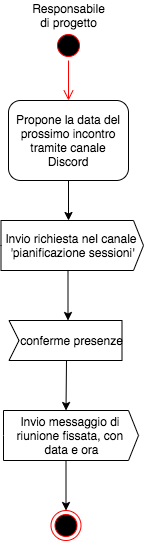
\includegraphics[width=3cm]{res/images/Riunione1.png}
	\caption{Organizzazione riunione interna}
	\label{fig:Organizzazione riunione interna}
\end{figure}
\textbf{Compiti dei partecipanti durante le riunioni:}
\begin{itemize}
\item{cercare di partecipare sempre attivamente alle riunioni: esporre le proprie perplessità affinchè i problemi vengano risolti subito;}
\item{cercare di essere presenti all'ora stabilita, nel caso di ritardi o impossibilità di presentarsi avvisare il Responsabile di Progetto;}
\item{comportamento corretto e linguaggio adeguato al contesto;}
\item{cercare di evitare rumori di sottofondo durante le riunioni telematiche per non creare disturbo agli altri componenti.}
\end{itemize}

\subsubsection{Riunioni esterne}
Una riunione è esterna quando a essa, oltre ai componenti del gruppo, partecipano il committente e/o il proponente.
Le riunioni esterne avvengono sempre in modalità telematica usando Zoom / Meet 
Nel caso di un ritorno alle modalità in presenza potrebbero essere fatte in locali universitari previo consenso da parte dei docenti, non nella sede dell'azienda essendo molto distante da Padova.
Per poter avere una riunione con il committente / proponente avvisarlo in anticipo di almeno 5 giorni.
Per poter avvisare il committente utilizzare la mail, per avvisare il proponente utilizzare Telegram.
\begin{figure}[H]
	\centering
	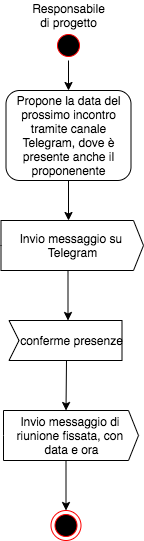
\includegraphics[width=3cm]{res/images/Riunione2.png}
	\caption{Organizzazione riunione esterna}
	\label{fig:Organizzazione riunione esterna}
\end{figure}

\subsection{Ruoli di progetto}
Tutti i ruoli saranno ricoperti da ciascun componente del gruppo in rotazione, secondo un calendario concordato, in modo che ogni membro possa assumere almeno una volta ciascuno di essi. All'incirca un ruolo dovrà essere mantenuto per circa 14 giorni, tempo necessario per poterlo ricoprire al meglio (per esempio il programmatore deve prima studiare il linguaggio e solo poi diventa effettivamente produttivo, quindi troppo pochi giorni non bastano).
Nel documento Piano di Progetto, vengono organizzate e pianificate le attività assegnate ai specifici ruoli previsti nell’attività di progetto. I Ruoli di Progetto sono:
\begin{itemize}
\item{\textbf{Responsabile di progetto;}}
\item{\textbf{Amministratore;}}
\item{\textbf{Analista;}}
\item{\textbf{Progettista;}}
\item{\textbf{Programmatore;}}
\item{\textbf{Verificatore;}}
\end{itemize}

\subsubsection{Responsabile di progetto}
Il Responsabile di Progetto,  o  “Project  Manager”,  è una figura essenziale e partecipa al  progetto per tutta la sua durata.  
\begin{itemize}
\item{Governa il team e rappresenta il progetto verso l'esterno}
	\begin{itemize}
	\item{accentra la responsabilità di scelta e approvazione;}
	\end{itemize}
\item{Ha responsabilità su:}
	\begin{itemize}
	\item{pianificazione;}
	\item{gestione delle risorse umane;}
	\item{controllo, coordinamento e relazioni esterne;}
	\item{approvazione della documentazione;}
	\item{approvazione dell’offerta economica;}
	\item{determinare e verificare le condizioni di completezza, ovvero quando il prodotto contiene tutti i requisiti richiesti dal committente e individuati dal gruppo.}
	\end{itemize}
\item{Deve avere conoscenze e capacità tecniche}
	\begin{itemize}
	\item{per valutare rischi, scelte, alternative.}
	\end{itemize}
\end{itemize}

\subsubsection{Amministratore di progetto}
L’ Amministratore è quella figura che ha il controllo sull'ambiente di lavoro. Inoltre ha diretta responsabilità sull'efficienza e sulla capacità operativa dell'ambiente di lavoro.
Ha in capo la redazione e la manutenzione migliorativa delle Norme di Progetto.
Egli:
\begin{itemize}
\item{controlla le versioni e le configurazioni del prodotto;}
\item{risolve i problemi legati alla gestione dei processi;}
\item{fornisce procedure e strumenti di monitoraggio/segnalazione, in modo da garantire un corretto controllo di qualità;}
\item{individua strumenti atti all’automazione dei processi, cioè studia e ricerca strumenti che riducano il più possibile l'impiego di risorse umane;}
\item{gestisce il versionamento della documentazione del progetto e della sua archiviazione.}
\end{itemize}


\subsubsection{Analista}
L’ Analista si occupa dell’analisi dei problemi e del \glock{dominio applicativo}. Svolge un ruolo fondamentale ai fini della riuscita del progetto, nonostante vi partecipi per un periodo di tempo limitato. Non segue il progetto fino alla consegna.
L'Analista redige l'Analisi dei requisiti e lo Studio di Fattibilità.
Egli:
\begin{itemize}
\item{si occupa dei documenti di Analisi dei requisiti e di Studio di Fattibilità;}
\item{conosce il dominio del problema e ha esperienza professionale;}
\item{ha molta influenza sul successo del progetto;}
\item{analizza il dominio applicativo:  gli utenti, l’ambiente d’uso.}
\end{itemize}


\subsubsection{Progettista}
Il Progettista è la figura che si occupa delle scelte architetturali del progetto e ne influenza gli aspetti tecnici e tecnologici, avendo competenze tecniche e tecnologiche aggiornate.
Utilizzando le attività svolte dall'Analista, il Progettista ha il compito di trovare una soluzione attuabile, comprensibile, chiara e motivata.
Egli:
\begin{itemize}
\item{produce una soluzione attuabile e chiara;}
\item{sviluppa l’architettura secondo un insieme di best practice per garantire coerenza e consistenza;}
\item{rende facilmente mantenibile il progetto;}
\item{definisce una struttura che abbia un basso grado di accoppiamento; un forte accoppiamento non è mai buona norma a meno che non si tratti di coesione;}
\item{sviluppa un’architettura solida,  sicura  e  flessibile, in modo  che rimanga funzionante in caso di malfunzionamenti e sia modificabile a basso costo;}
\item{applica soluzioni note e ottimizzate.}
\end{itemize}

\subsubsection{Programmatore}
Il Programmatore è il responsabile della codifica del progetto e delle componenti di supporto, che serviranno per effettuare le prove di verifica e validazione sul prodotto.
Partendo dall’attività del Progettista, il Programmatore realizza l’architettura già definita con l’unica responsabilià di svolgere al meglio il lavoro già progettato.
Egli:
\begin{itemize}
\item{implementa in maniera precisa e scrupolosa le soluzioni generate dal Progettista;}
\item{scrive codice sorgente altamente e facilmente manutenibile;}
\item{una volta terminata la codifica, se il prodotto realizzato non è di facile utilizzo può redigere un Manuale Utente;}
\item{si occupa anche del versionamento e della documentazione del codice sorgente.}
\end{itemize}

\subsubsection{Verificatore}
È una figura presente per tutta la durata del progetto. Ha competenze tecniche, esperienza professionale e conoscenza del \glock{way of working}.	
Redige la parte retrospettiva del Piano di Qualifica che illustra l'esito e la completezza delle verifiche e delle prove effettuate secondo il piano.
Egli:
\begin{itemize}
\item{assicura che nel corso del progetto vengano rispettate le norme redatte in questo documento di Norme di Progetto;}
\item{assicura che ogni stadio del ciclo di vita del prodotto sia conforme al Piano di Qualifica.}
\end{itemize}


\subsection{Formazione del personale}
Per quanto riguarda la formazione, i membri del gruppo DPCM 2077 devono procedere in modo autonomo con lo studio individuale delle tecnologie che verranno utilizzate nel corso del progetto, prendendo come materiale di riferimento quello indicato nella sezione sezione \textbf{Riferimenti Informativi}. Si è comunque deciso di avere all'interno del Team un esperto di Git e {\LaTeX}, in modo che nel caso di ambiguità o difficoltà nell'utilizzo i componenti possono direttamente
rivolgersi a queste persone. Con lo studio autonomo poi si possono aiutare i componenti che si trovano magari in difficoltà con qualche strumento o tecnica, dando origine così a un miglioramento continuo per tutti e ad un'efficienza e qualità maggiore nelle attività. 



\subsection{Ambiente di lavoro}

\subsubsection{Ticketing}
Per assegnare le varie attività da svolgere tra i componenti del gruppo DPCM 2077 si è scelto di ricorrere all'\glock{Issue Tracking System} (ITS) di GitHub.
Quando una \glock{issue} viene assegnata a un componente del gruppo, automaticamente gli viene inviata una e-mail.
Quando si va a creare una issue, bisogna compilare i seguenti campi:
\begin{itemize}
\item{\textbf{title}: indica il titolo dell'attività da svolgere o criticità da risolvere, nel caso della stesura di un documento il titolo deve corrispondere al nome del documento;}
\item{\textbf{leave a comment}: area di testo dove è possibile specificare meglio la descrizione della issue;}
\item{\textbf{assignees}: indica il componente o i componenti ai quali viene assegnato il task da svolgere o la criticità da risolvere;}
\item{\textbf{labels}: indica le etichette che vengono associate alla issue, per esempio: bug, documentation, help wanted;}
\item{\textbf{milestone}: specifica a che Milestone è associata la issue che si sta creando.}
\end{itemize} 
\begin{figure}[H]
	\centering
	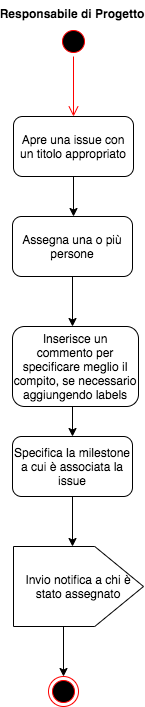
\includegraphics[width=3cm]{res/images/ticket.png}
	\caption{Assegnazione di un ticket}
	\label{fig:Assegnazione di un ticket}
\end{figure}

\subsubsection{Coordinamento attività}
\begin{description}
\item{\textbf{Versionamento}}: per il versionamento si è deciso di utilizzare Git, poiché conosciuto da tutti i membri del gruppo DPCM 2077 grazie anche all'insegnamento offerto
nel Corso di Laurea \textbf{Tecnologie Open Source} frequentato da tutti i componenti. Con Git è incentivato lo sviluppo su \glock{branch} diversi che possono essere locali o condivisi.
La maggior parte delle operazioni viene fatta in locale, i requisiti primari sono la velocità e le performance.
Possono essere adottati diversi tipi di \glock{Workflow} e ogni commit è identificato da un ID che ne garantisce l'integrità.
Non è possibile cambiare un commit senza modificare l’ID del commit stesso e dei i commit successivi.  
Si è stabilito inoltre di appoggiarsi al servizio di hosting GitHub per la sua interfaccia intuitiva e per l' Issue Tracking System integrato che offre molteplici funzionalità

\item{\textbf{Pianificazione delle attività}}:  per la pianificazione delle attività il gruppo ha deciso di utilizzare il software \textbf{\glock{GanttProject}}. 
È un programma completamente scritto in linguaggio Java e sotto licenza GPL, quindi gratuito e liberamente utilizzabile, che permette di pianificare ogni tipo di progetto o attività utilizzando la tecnica di Gantt.
Può essere utilizzato sui principali sistemi operativi, quali: Windows, macOS e Linux.
È quindi possibile:
\begin{itemize}
\item{\textbf{creare l'elenco delle attività per il progetto:} data, ora di inizio e priorità;}
\item{\textbf{determinare i tempi necessari per le singole attività;}}
\item{\textbf{salvare spesso il progetto;}}
\item{\textbf{annullare le ultime operazioni in caso di errore;}}
\item{\textbf{generare diagrammi PERT:} per le dipendenze temporali fra attività e evidenziando le loro criticità;}
\end{itemize} 

\item{\textbf{Continuous Integration}}:  per la Continuos Integration il team ha preso in considerazione i seguenti strumenti: \glock{\textbf{TravisCI}}, \glock{\textbf{Jenkins}} e \glock{\textbf{GitHub Actions}};
Si è deciso in seguito di utilizzare GitHub Actions in quanto direttamente integrato nel sistema di versionamento utlizzato e perchè 
GitHub offre modelli di workflow CI per una varietà di linguaggi e framework.
Non è stato immediatamente scartato TravisCI in quanto già conosciuto da parte dei membri del team, ma non integrato su GitHub tanto quanto GitHub Actions.
La Continuos Integration che utilizza GitHub Actions offre workflow che possono creare il codice nel repository ed eseguire i test. 
I workflow possono essere eseguiti su macchine virtuali ospitate da GitHub o su macchine ospitate personalmente.
GitHub esegue i test di CI e fornisce i risultati di ogni test nella richiesta \glock{pull}, così è possibile vedere se la modifica di un ramo introduce un errore. 
Quando tutti i test CI in un workflow vengono superati, le modifiche inviate sono pronte per essere riviste da un membro del team. 
Quando un test fallisce, una delle modifiche apportate potrebbe aver causato il fallimento. 

\end{description}

\subsubsection{Documentazione} 
\begin{description}
\item{\textbf{\LaTeX}}: è un programma professionale di composizione tipografica multilingua,
multipiattaforma e completamente gratuito. Permette di produrre documenti in formato pdf di elevata qualità, adatti sia per la stampa digitale, sia
per la pubblicazione e la consultazione on-line. 
Altri strumenti come Google Docs e LibreOffice per la scrittura di documenti sono stati scartati in quanto non adeguati per scrivere documenti ufficiali per il progetto.

\item{\textbf{Editor}}: l’editor  consigliato  per  scrivere  la  documentazione  con  {\LaTeX}  è TexStudio  in  quanto  software  libero  aggiornato  e  multi  piattaforma. Per piattaforma macOS è invece disponibile
anche l'editor TeXShop. Entrambi i programmi una volta compilati i file .tex producono in automatico un file .pdf con il documento.

\item{\textbf{Diagrammi UML}}: per modellare con UML è stato deciso di utilizzare il software StarUML. È uno strumento per creare diagrammi delle classi e altri tipi di diagrammi secondo Unified Modeling Language (UML). 
Viene anche utilizzato per la generazione automatica di codice Java a partire dalla sua rappresentazione UML; è possibile, inoltre, effettuare l’operazione inversa (reverse engineer) del codice Java sorgente per produrre il diagramma UML corrispondente. 
\end{description}

\subsubsection{Ambiente di sviluppo}
\begin{description}
\item{\textbf{Sistemi Operativi}}: i membri del gruppo DPCM 2077 potranno lavorare sui principali sistemi operativi presenti nel mercato, cioè: Windows, macOS e Linux.
I principali strumenti e programmi richiesti sono ormai presenti in tutti e tre i sistemi operativi.
\item{\textbf{Ambienti integrati di sviluppo}}
\begin{enumerate}
\item{\textbf{WebStorm}}: WebStorm è un IDE di grande valore per chi sviluppa con Javascript per alcuni semplici motivi, elenchiamo i principali:
\begin{itemize}
\item WebStorm è pieno di funzioni interessanti di auto-completamento;
\item controllo della sintassi e adeguamento alle varie versioni del linguaggio;
\item WebStorm è in grado di supportare TypeScript.
\end{itemize}
Ci sono anche altri lati positivi di WebStorm, ad esempio quelli che sono inerenti alle funzioni di refactoring del codice e ovviamente all’integrazione con i sistemi di versioning.
\item{\textbf{PyCharm}}: È particolarmente utile per chi sviluppa in Python perché integra diverse funzionalità utili nel development, alcuni esempi:
\begin{itemize}
\item il completamento della sintassi delle istruzioni;
\item l'help online;
\item l'evidenziazione degli errori di sintassi durante lo sviluppo;
\item la console di Python in una finestra dell'editor.
\end{itemize}
\end{enumerate}
\end{description}

\subsection{Strumenti organizzativi}
Il gruppo nel corso del progetto ha utilizzato e utilizzerà i seguenti strumenti:
\begin{itemize}
\item{\textbf{Telegram}}: strumento di messaggistica utilizzato inizialmente per la gestione del gruppo;
\item{\textbf{GitHub}}: per il versionamento e il salvataggio in remoto di tutti i file riguardanti il progetto; 
\item{\textbf{Google Drive}}: utilizzato per il salvataggio di grafici, tabelle e per una gestione generale del progetto;
\item{\textbf{Discord}}: utilizzato come canale principale per le comunicazioni tra i membri del gruppo.
\end{itemize}
